\chapter{Угадыватель чисел}
\label{ch:guessnumbers}

В этой главе мы познакомим вас с программой <<Угадыватель чисел>>\cite{PanfilovaApp}, идея которой взята из книги Л. Ф. Магницкого «Арифметика»\cite{Galanin}. 
Опишем задачу и расскажем, как запрограммировать решение. Поработаем с экранами приложения, создадим процедуры и покажем как разрешить ввод только числовых значений в программе.


\section{Описание задачи}

Суть предлагаемой нами задачи описана в книге Л. Ф. Магницкого, «Арифметика», в главе: «Об утешных некиих действиях, через арифметику употребляемыx»\cite{Galanin}.

Пронумеруем дни недели от одного (понедельник) до семи (воскресенье). 
Предложим игроку загадать число, равное номеру любого дня недели. Далее попросим загадавшего выполнить следующие действия:
\begin{enumerate}
\item Умножить номер загаданного дня недели на два\footnote[][-0cm]{Шаг 1.}\marginnote[0.2cm]{Пусть $ a $ — искомое число (день недели), $ a \in [1;7] $. В результате выполнения шага 1 получаем $2\cdot a $}. 
\item К полученному произведению прибавить пять\footnote[][-0cm]{Шаг 2.}\marginnote[0.2cm]{$2\cdot a + 5$}.
\item Затем полученную сумму умножить на пять\footnote[][-0cm]{Шаг 3.}\marginnote[0.2cm]{$5\cdot(2 \cdot a  + 5) = 10 a + 25$}.
\item Полученное число умножить на десять\footnote[][-0cm]{Шаг 4.}\marginnote[0.2cm]{$(10a + 25)\cdot 10 = 100  a + 250$}.
\item Назвать результат вычислений.
\end{enumerate}

Чтобы перейти от полученного числа к загаданному, необходимо вычесть из него двести пятьдесят и поделить полученное число на сто\footnote[][-0cm]{Определяем число, загаданное игроком: $\frac{100  a + 250 - 250}{100} =  a $}. 

Таким образом, с помощью этих арифметических преобразований мы определили, какое число загадал игрок, то есть нашли~$a$.
\begin{mdfstyle}[nobreak=true,frametitle=Вопрос о числовых множествах]
  \sloppy 
  При постановке задачи мы указали, что а это номер дня недели, то есть натуральное число, $ a \in \mathbb{N} $ . Будет ли работать наш алгоритм угадывания для чисел из множеств $\mathbb{Z}, \mathbb{Q}, \mathbb{R} $? И что это за множества?  
  Ответ на странице \pageref{answer:guess_numbers_task}.
  \label{question:text}
\end{mdfstyle}

\section{Реализация приложения}
\label{styles}
В программе «Угадыватель чисел» (The Numbers Guessing Game)\cite{PanfilovaApp} загаданный игроком номер дня недели — это то, что мы будем искать.
Создадим глобальную переменную  \textit{SecretNumber} для хранения искомого числа, загаданного игроком. Присвоим этой переменной значение, равное нулю. 
Так как ноль не входит в интервал от одного до семи, то переменная \textit{SecretNumber} в данный момент не равна загаданному числу $ a $\footnote[][-0cm]{\mbox{$ \left.\begin{array}{ccc}
  SecretNumber = 0 \\
  a \in [1;7] \\
\end{array}
\right\}\Rightarrow SecretNumber \neq a $}}. Это хороший стиль программирования, который позволяет проинициализировать переменную так, чтобы явно указать, что результат ещё не получен. Также
отметим, что в этом приложении объекты именуются в стиле PascalCase\cite{Chase2018}\marginnote[0.2cm]{Именовать объекты можно также произвольно, но рекомендуется использовать один из общепринятых стилей.
  Существуют следующие стили написания составных слов: CamelCase, SnakeCase, KebabCase, PascalCase и другие.
  Подробнее о них можно узнать в статье Чейза Адамса <<Стили написания составных слов в программировании>>}.

\subsection{Определение числа, загаданного игроком}
Чтобы в поле \textit{NumberText} пользователь мог вводить только числовые значения, необходимо поставить галочку у свойства \textit{NumbersOnly} этого поля.

Рассмотрим блок обработки нажатия (рис.~\ref{fig:block:button:click}) на кнопку «Узнать ответ» (Button1).
Когда игрок нажимает на эту кнопку, последовательно выполняются следующие действия:
\begin{figure}
  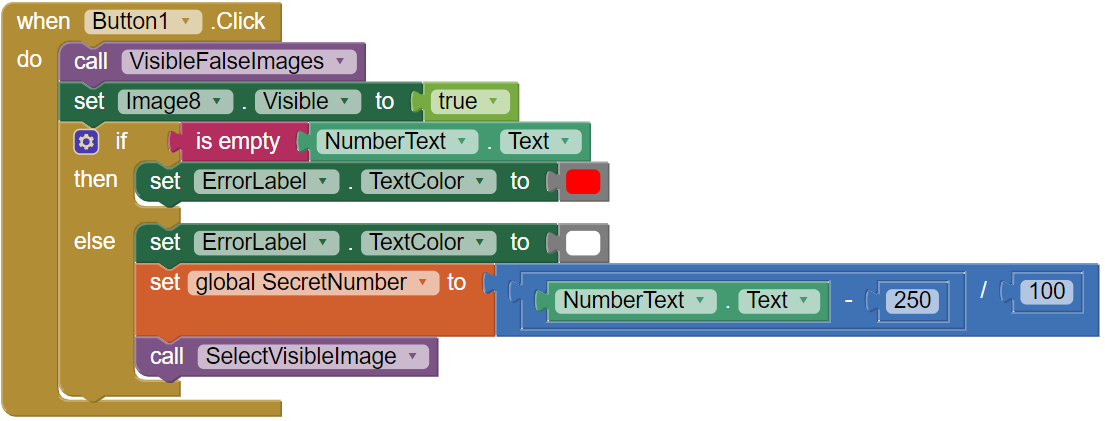
\includegraphics{./graphics/programs/guess_numbers/block_Button1Click_AppInventor_2018.png}
    \caption[Блок обработки нажатия на кнопку Button1.][12pt]{Блок обработки нажатия на кнопку Button1 и сокрытия всех изображений цифр, вывод результата или сообщения об ошибке.}
  \label{fig:block:button:click}
\end{figure}
\begin{enumerate}
  \item Вызываетcя процедура \textbf{VisibleFalseImages} (рис.~\ref{fig:block:visible:false:images}), которая устанавливает свойство Visible у всех изображений с цифрами в false. Таким образом, пока не будет определено число, загаданное пользователем, изображения с цифрами не будут отображаться.
  \begin{marginfigure}[-2em]
    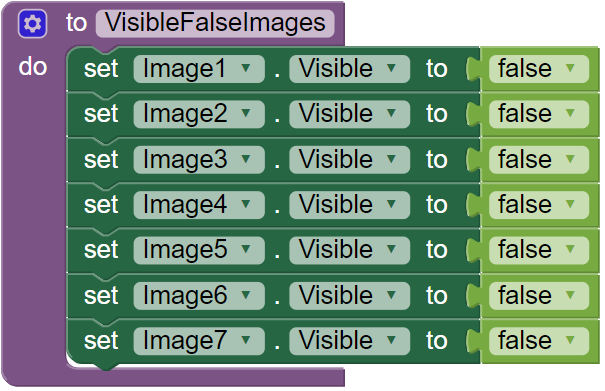
\includegraphics{./graphics/programs/guess_numbers/procedure_visibleFalseImages_AppInventor_2018.png}
      \caption[Процедура VisibleFalseImages.]{Процедура VisibleFalseImages устанавливает свойство Visible у всех изображений с цифрами в false.}
    \label{fig:block:visible:false:images}
  \end{marginfigure}

  \item Устанавливается свойство \textit{Visible} в значение true у изображения со знаком вопроса (Image8).
  \item Если значение поля для ввода загаданного числа (\textit{NumberText}) пусто, то приложение сигнализирует пользователю об ошибке следующим образом. Устанавливаем красный цвет шрифта, чтобы стало видно сообщение «Пожалуйста, введите полученное число» у поля \textit{ErrorLabel} (рис.~\ref{fig:display:error}).
  \begin{marginfigure}[2em]
    
\includegraphics{./graphics/programs/guess_numbers/finalScreen_Error2_TheGuessingNumbersGame_AppInventor.jpg}
      \caption[Сообщение об ошибке на экране FinalScreen.]{Сообщение об ошибке на экране FinalScreen.}
    \label{fig:display:error}
  \end{marginfigure}
  В случае, когда что-либо введено в поле \textit{NumberText}, последовательно выполняются следующие шаги:
  \begin{itemize}
    \item Устанавливается белый цвет шрифта у поля \textit{ErrorLabel}, чтобы скрыть сообщение об ошибке.
    \item Производится подсчёт значения переменной \textit{SecretNumber}.
    \item Вызывается процедура \textbf{SelectVisibleImage}, которая будет рассмотрена далее.
  \end{itemize}
\end{enumerate}
Возникает вопрос: почему для того, чтобы отображать сообщение об ошибке мы меняем цвет текста у поля \textit{ErrorLabel}, а не управляем значением свойства \textit{Visible}? 
Дело в том, что при использовании свойства \textit{Visible}, любое изменение его значения вызывает перерисовку экрана, а элементы интерфейса будут менять свои позиции, то есть <<скакать>> по экрану.
В нашем приложении, если цвет поля белый, то компонент \textit{ErrorLabel} сливается с фоном экрана, сообщения об ошибке не видно.
\section{Процедура SelectVisibleImage}

\begin{figure}
  \includegraphics{./graphics/programs/guess_numbers/procedure_selectVisibleImage_AppInventor_2018.png}
    \caption[Процедура SelectVisibleImage.]{Процедура SelectVisibleImage управляет отображением изображений с цифрами. Пунктирной линией отреза сокращено число однотипных блоков управления, выполняющих действия по установке значения свойства Visible в true у изображения с числом, которое соответствует значению переменной \textit{SecretNumber}. На рисунке такие блоки указаны для чисел один и семь.}
  \label{fig:block:click:select:visible:image}
\end{figure}

Процедура \textbf{SelectVisibleImage} (рис.~\ref{fig:block:click:select:visible:image}) читает значение глобальной переменной \textit{SecretNumber} и отображает рисунок с соответствующей цифрой.
В случае, если число не было определено, показывается изображение с вопросительным знаком (\textit{Image8}).

Например, пусть игрок загадал число три. На основании введённого пользователем числа в поле \textit{NumberText} на экране \textit{FinalScreen}
(пусть в этом примере введено число 550)\footnote[][0.5cm]{ Пусть $ x $ — число, которое должен ввести пользователь, $ a $ — загаданный игроком номер дня недели, $ a \in [1;7] $, $ ] a = 3 $. 

Чтобы найти $ x $ выполним следующие преобразования:

$ x = 100 \cdot a + 250  = 100 \cdot 3 + 250  = 550 $}\marginnote[0.2cm]{} приложение подсчитает и присвоит переменной \textit{SecretNumber} новое значение, равное трём.
Процедура \textit{SelectVisibleImage} в соответствии со значением переменной \textit{SecretNumber} делает видимым изображение с соответствующей загаданному числу цифрой. 
В нашем примере это изображение числа три (\textit{Image3}). Если переменная \textit{SecretNumber} содержит значение, не входящее в интервал от одного до семи, то будет показано изображение со знаком вопроса (\textit{Image8}), а текст надписи \textit{ErrorСalculating} станет видимым (<<Допущена ошибка в расчетах. Попробуйте снова>>, рис.~\ref{fig:block:final:screen:error:label}).
\begin{marginfigure}[-2em]

\includegraphics{./graphics/programs/guess_numbers/finalScreen_Error_TheGuessingNumbersGame_AppInventor.jpg}
\caption[Сообщение об ошибке в расчётах на экране FinalScreen.]{Сообщение об ошибке в расчётах на экране FinalScreen.}
  \label{fig:block:final:screen:error:label}
\end{marginfigure}
Важно отметить, что перед выполнением орпераций сравнения переменной \textit{SecretNumber} с введенным пользователем числом, выполняется установка свойства \textit{Visible} в \textit{false} у элементов \textit{Image8} и \textit{ErrorСalculating} (рис.~\ref{fig:block:click:select:visible:image}).
Тем самым мы отмечаем отсутствие ошибок в вычислениях и заранее убираем с экрана знак вопроса, предполагая, что на его месте будет изображение с определённой цифрой. Если же переменная \textit{SecretNumber} не входит в интервал от одного до семи, то у элементов \textit{Image8} и \textit{ErrorСalculating} устанавливается значение свойства \textit{Visible} в \textit{true}, 
так приложение сообщает пользователю о его ошибке в вычислениях.

\subsection{Работа с экранами}
При проектировании приложения были учтены рекомендации из официальной документации App Inventor\cite{MitManyScreens} по ограничению количества экранов во избежание проблем с переполнением памяти.
Поэтому в игре используется восемь экранов (рекомендуемое количество — меньше 10):
\begin{enumerate}
\item \textbf{Screen1} — главный экран приложения, меню игры.
\item \textbf{About} — экран, содержащий информацию о приложении.
\item \textbf{Step1}, \textbf{Step2}, \textbf{Step3}, \textbf{Step4}, \textbf{Step5} — это экраны с пошаговым описанием задания пользователю. На экранах есть следующие кнопки для навигации между экранами приложения:
\begin{itemize}
  \item «\textit{На шаг назад}» (\textit{PreviousStepButton}) меняет экран на предыдущий.
  \item «\textit{Далее}» (\textit{NextStepButton}) — переход игрока на следующий экран.
  \item «\textit{В главное меню}» (\textit{BackToMainMenuButton}) показывает пользователю главный экран \textit{Screen1}.
\end{itemize}
\item \textbf{FinalScreen} — это экран с результатами игры. Здесь пользователю необходимо ввести получившееся в результате вычислений число и нажать кнопку «\textit{Узнать ответ}» (рис.~\ref{fig:block:final:screen:error:label}), чтобы увидеть на экране число, которое по предположению программы загадал игрок.
\end{enumerate}

\begin{mdfstyle}[nobreak=true,frametitle=Упражнение]
\sloppy Приложение можно перепроектировать таким образом, чтобы экраны \textit{Step1}, \textit{Step2}, \textit{Step3}, \textit{Step4}, \textit{Step5} представляли собой один экран. Попробуйте реализовать приложение «Угадыватель чисел» с одним общим экраном \textit{Steps}, в котором пользователю будет предложена пошаговая инструкция по преобразованию загаданного числа. Общий экран \textit{Steps} будет для этого включать навигационные кнопки.\end{mdfstyle}

Если вызывать блок управления среды App Inventor для открытия другого экрана \textit{``open another screen''}, а затем не вызывать блок управления для закрытия экрана \textit{``close screen''}, то через некоторое время приложение израсходует всю доступную память.
Рассмотрим решение этой проблемы в нашем приложении. Экран \textit{Screen1} содержит в себе элементы интерфейса для отображения названия игры и две кнопки: «\textit{Старт}» (\textit{StartButton} для перехода на экран \textit{Steps}) и «\textit{Об игре}» (\textit{AboutButton} для перехода на экран \textit{About}). Для того, чтобы не получить ошибку переполнения памяти, создадим процедуру для закрытия экрана, которую назовём \textbf{CloseScreen} (рис.~\ref{fig:block:click:close:screen}). Она будет содержать в себе один единственный блок управления «\textit{close screen}». 
\begin{marginfigure}[-2em]
  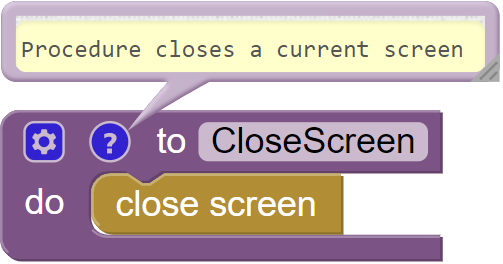
\includegraphics{./graphics/programs/guess_numbers/procedure_closeScreen_AppInventor_2018.png}
    \caption[Процедура CloseScreen.]{Процедура CloseScreen закрывает текущий экран.}
  \label{fig:block:click:close:screen}
\end{marginfigure}
Возникает вопрос: зачем действие по закрытию экрана помещать в отдельную процедуру? Это необходимо для того, чтобы последовательно выполнить блоки управления \textit{``open another screen''} и \textit{``close screen''} при возникновении события нажатия на любую навигационную кнопку (\textit{Click}). «Пазлы» блоков управления открытия и закрытия экрана спроектированы так, что их нельзя объединить в одном блоке App Inventor, но можно соединить их через вызов процедуры, что и было сделано (рис.~\ref{fig:block:click:close:screen}).
